\chapter{Fundamentação Teórica} \label{CHP:FUND}

\section{Serviços PaaS}
\subsection{Definição}

Segundo o \ac{NIST}, o termo computação em núvem tem a seguinte definição: ``Cloud Computing (pt: computação em nuvem) é um modelo que permite, de forma conveniente, o acesso à rede sob demanda para um conjunto compartilhado de recursos de computação configuráveis (por exemplo, redes, servidores, armazenamento, aplicativos e serviços) que podem ser rapidamente provisionados e lançados  com o mínimo de esforço de gestão ou a interação de um prestador de serviços.''. Um dos serviços definidos é o \ac{PaaS}.

	Ainda de acordo com o \ac{NIST}, o \ac{PaaS} é ``a capacidade fornecida ao consumidor de publicar aplicações usando linguagem de programação, bibliotecas, serviços suportados pelo provedor''. Com o fornecimento de tal serviço, o consumidor não precisa se preocupar com o controle de certos serviços de infra-estrutura, como a rede, servidores, sistemas operacionais, armazenamento, ou seja, criam uma camada de abstração de serviços de infra-estrutura.
	
	De acordo com \cite{cloudstack}, serviços \ac{PaaS} possuem as seguintes características:
\begin{itemize}
\item Serviços para desenvolver, testar, publicar, hospedar e manter aplicações de forma integrada;
\item Arquitetura Multi-tenant, onde vários usuários podem utilizar o mesmo ambiente de desenvolvimento;
\item Construção garantindo escalabilidade, incluindo balanceamento de carga (load balancing) e replicação de dados para recuperação de falhas (failover);
\item Integração com web services e banco de dados através de padrões comuns;
\item Suporte para desenvolvimento em equipes, podendo ter ferramentas de planejamento de projetos e de comunicação;
\item Ferramentas para gerenciamento dos custos.
\end{itemize}

	Ou seja, sistemas \ac{PaaS} são úteis para desenvolvedores individuais e startups\footnote{Termo utilizado para designar modelo de négocios repetível e escalável, em um ambiente de extrema incerteza. Normalmente, projetos ou empresas startups estão associadas as áreas de tecnologia.}, pois fornecem facilidade de publicação sem os custos e complexidades de hardwares e softwares inerentes a uma aplicação web comum \cite{guardianstartup}.
	
\subsection{Heroku}

	O \emph{Heroku} é uma plataforma cloud de serviços \ac{PaaS} montado sobre o \emph{Amazon EC2}, existente desde junho de 2007. Possui suporte para as seguintes linguagens: Ruby, Java, Node.JS, Scala, Clojure, Python e PHP. Internamente, funciona sobre o sistema operacional Ubuntu.

	Inicialmente, o \emph{Heroku} foi desenvolvido com suporte exclusivo para a linguagem Ruby. Em julho de 2011, Matz Matsumoto, criador do Ruby, entrou para a empresa como Arquiteto-chefe e, nesse mesmo mês, passou a dar suporte também para Node.js e Clojure.
Em setembro de 2011, a rede social \emph{Facebook} fez uma parceria com o \emph{Heroku} a fim de facilitar a publicação de aplicativos para sua própria plataforma \cite{faceheroku}. Em poucos passos, é possível criar uma aplicação no Facebook e no Heroku, simultaneamente.
O \emph{Heroku} usa uma unidade de máquina virtual chamada ``Dyno'' com 4 cores e até 512mb de RAM.

	

\section{REST}
 O \ac{REST} foi definido em uma tese de doutorado por Roy Fielding da seguinte maneira: 
``O \ac{REST}  é pretendido como uma imagem do design da aplicação se comportará: uma rede de websites (um estado virtual), onde o usuário progride com uma aplicação selecionando as ligações (transições do estado), tendo como resultado a página seguinte (que representa o estado seguinte da aplicação) que está sendo transferida ao usuário e apresentada para seu uso.''

	De modo geral, o \ac{REST} é uma interface de comunicação onde há um provedor de serviços e um consumidor. Tal interface pode ser descrita utilizando \ac{XML}, \ac{HTTP}, \ac{YAML}, \ac{JSON} ou até mesmo texto puro, de modo a não utilizar trocas de mensagens complexas como o \ac{SOAP}. 

O \ac{REST} possui alguns princípios, a saber:
\begin{itemize}
\item Modelo provedor/consumidor stateless (sem estado): cada mensagem \ac{HTTP} trocada possui todas as informações necessárias para a comunicação, ou seja, nenhuma das partes necessita gravar estado da comunicação. Em sistemas web, é comum o uso de cookies para manter o estado da sessão; já em sistemas mobile, é comum utilizarmos um token de autenticação, com a mesma finalidade.

\item Operações \ac{HTTP}: de modo a diminuir o tráfego de dados, são utilizados métodos \ac{HTTP} para acessar os recursos de informação. As operações mais utilizadas são o \emph{GET}, \emph{PUT}, \emph{POST} e \emph{DELETE}. Em sistemas \ac{REST}, é comum combinar tais métodos com operações de \ac{CRUD}, que faz persistência de dados em um determinado recurso ou entidade.

\item Identificação de recursos: As URLs identificam cada uma das entidades e seus elementos, ficando a cargo da operação \ac{HTTP} definir a ação a ser feita com cada um dos recursos ou elementos.

\item Uso de hipermídia: As trocas de mensagem de comunicação é feita utilizando, no corpo da mensagem \ac{HTTP}, uma linguagem de marcação, conforme já citado anteriormente. Porém, não há uma restrição geral quanto ao uso, podendo ser usada linguagens próprias (texto puro).

\end{itemize}
\subsection{RESTful}

	Em uma arquitetura julgada como \emph{RESTful}, o método desejado é informado dentro do método \ac{HTTP}, contido no header do mesmo. Além disso, o escopo da informação é colocado na \ac{URL}, o que torna uma ``combinação poderosa''. Por definição, uma aplicação deixa de ser RESTFul caso o método \ac{HTTP} não combine com o método da informação, ou seja, com a funcionalidade esperada para aquela estrutura de dados. \cite{restfulws}

\section{JSON}
\subsection{Introdução}
\ac{JSON} é um padrão aberto de texto para representar estruturas de dados, de forma inteligível para humanos.  Sua origem é a linguagem javascript, e seu formato está descrtio no RFC 4627.

\subsection{Definição}
	O \ac{JSON} é um dos formatos mais usados na serialização e transmissão de dados estruturados pela internet,ao lado do \ac{XML} e \ac{YAML}, sendo muito usado em sistemas orientados a serviço e/ou web services. Muitas linguagens e \emph{frameworks}, como o Foundation (iOS) e o Android, dão suporte para esse padrão, através de parsers\footnote{Em português, parsers são analisadores sintáticos que analisam uma sequência de entrada para determinar sua estrutura gramatical segundo uma determinada gramática formal.} para construção e consumo.
	
De acordo com \cite{restfulws}, ``é muito mais fácil para um browser lidar com uma estrutura javascript oriunda de uma estrutura \ac{JSON} do que a partir de um documento \ac{XML}''. Ainda de acordo com a fonte, cada web browser oferece uma interface JavaScript diferente para seus parsers \ac{XML}, enquanto um objeto \ac{JSON}, que por definição é um objeto JavaScript, será interpretado da mesma maneira em qualquer interpretador JavaScript. O \ac{JSON} é uma alternativa mais leve para serialização de dados do que o \ac{XML}, definido pelo \ac{XML} Schema. 

\subsection{comparação com XML}
	\ac{JSON} e \ac{XML} são dois formatos de manipulação de informações que podem ser usados com o mesmo objetivo, mas possuem implementações e aplicações distintas. 

	No artigo \cite{comparexmljson}, é feito um estudo considerando a hipótese de que não há diferença em relação ao tempo de transmissão e os recursos utilizados entre \ac{JSON} e \ac{XML}.A fim de realizar o estudo, foi criado um ambiente operacional consistindo de uma aplicação cliente/servidor em Java, onde o servidor escuta uma porta e o cliente conecta a ela. 

	No referido teste, foram utilizadas as seguintes métricas: número de objetos enviados, tempo total para enviar o número de objetos, tempo médio de transmissão, uso da CPU pelo usuário, uso da CPU pelo sistema e o uso de memória.

	De acordo com a conclusão do artigo, codificação \ac{JSON} é, em geral, mais rápida e consome menos recursos que a codificação \ac{XML}, o que nega a hipótese de igualdade de escolha entre as duas tecnologias. Ou seja, em um ambiente onde é necessária velocidade e os recursos são limitados, como sistemas móveis, é preferível utilizar \ac{JSON}.

\subsection{Estrutura}
	De acordo com W3resource \cite{w3json}, o \ac{JSON} suporta duas grandes estruturas de informação: coleção de pares chave/valor e listas ordenadas de valores. Ambas estruturas são também suportadas pela maioria das linguagens de programação modernas, o que reforça a ideia de ser uma boa escolha de linguagem para transmissão de informações.
	
	O \ac{JSON}possui alguns tipos de dados, a saber:
\begin{itemize}
\item Objetos: um objeto começa e termina com '{' e '}', contendo um número de pares chave/valor.  A separação entre uma chave e um valor é feita com o caractere ':',  e a separação entre pares é feita com ','. O valor de um par pode ser qualquer estrutura \ac{JSON}.
\item Arrays: Um array começa e termina com '[' e ']'. Entre eles, são adicionados certo numero de valores, separados por ','. 
\item Valores: os valores podem ser string, número, objeto, array, valor booleano ou nulo.
\end{itemize}
Exemplo de código \ac{JSON}:

\begin{lstlisting}
{
    "firstName": "Bidhan",
"lastName": "Chatterjee",
    "age": 40,
    "address": {
        "streetAddress": "144 J B Hazra Road",
        "city": "Burdwan",
        "state": "Paschimbanga",
        "postalCode": "713102"
    },
    "phoneNumber": [
        {
            "type": "personal",
            "number": "09832209761"
        },
        {
            "type": "fax",
            "number": "91-342-2567692"
        }
    ]
}
\end{lstlisting}

\section{Ruby on Rails}

\subsection{Ruby}
	Ruby é uma linguagem orientada a objetos, com tipagem forte e dinâmica, criada por Yukihiro Matsumoto (Matz) em 1995. 
	
	Segundo \cite{caelum}, uma de suas principais características é sua expressividade, ou seja, a facilidade de ser lida e entendida, o que facilitaria o desenvolvimento de sistemas escritos por ela.
	
	O livro \cite{rails3} lista algumas das características mais importantes do Ruby, a saber:
\begin{itemize}
\item É uma linguagem interpretada, ou seja, um interpretador lê o código e decide como executar em tempo de execução. Por consequência, um sistema em Ruby pode se tornar um pouco mais lento, porém, é notável o ganho em flexibilidade.
\item Possui uma sintaxe de linguagem flexível, fazendo com que a curva de aprendizado seja menor em relação a outras linguagens. Um exemplo clássico é a não-necessidade (opcional) de escrever parênteses ao redor dos parâmetros de um método. Entretanto, podem surgir erros misteriosos por não colocar parênteses em algumas situações ambíguas.
\item Possui uma tipagem dinâmica, ou seja, não é necessário especificar o tipo de informação que será guardado em cada variável. Isso torna a abordagem bem mais flexível, tornando as operações dependentes do próprio contexto. Entretanto, problemas podem ocorrer justamente por isso: comportamentos inesperados.
\item Suporte a blocos e closures,
\end{itemize}
	
	Atualmente, Ruby encontra-se entre as linguagens de programação mais populares, ocupando a posição 11º no índice Tiobe\footnote{O índice TIOBE mede, mensalmente, a popularidade de uma determinada linguagem de programação, baseado no numero de engenheiros qualificados, cursos, vendedores e buscas nos principais motores de busca. Pode ser encontrado em \url{http://www.tiobe.com/index.php/content/paperinfo/tpci/index.html} }.  Grande parte desse sucesso deve-se ao \emph{framework} Rails, implementado como solução web utilizando Ruby.

\subsection{Rails}
	O Ruby on Rails, também chamado Rails ou RoR, é um \emph{framework} de desenvolvimento web de código aberto que tem como premissa aumentar a velocidade e a facilidade no desenvolvimento de aplicações web orientados a banco de dados.  Foi lançado oficialmente em Julho de 2004 pelo seu criador David H. Hansson, estando atualmente na versão 3.2.11, com a 4ª versão em desenvolvimento \cite{rails4}.  
	
	O Rails é um \emph{framework} \emph{full-stack}, ou em português, pilha completa. Isso significa que, com ele, é possível desenvolver a aplicação por completo, desde o desenvolvimento dos layouts das paginas, a manutenção do banco de dados. Além disso, o Rails enfatiza o uso de alguns padrões de engenharia de software, a saber:
	
\begin{itemize}
\item Active record: padrão de projeto para armazenamento de dados em banco de dados relacionais.  A interface de um certo objeto deve incluir funções de \ac{CRUD},  como inserir, atualizar, apagar e algumas funções de consulta. Cada tabela de um banco de dados é ``envelopada''  em um uma classe, sendo cada instancia dessa classe um registro (tupla) único na tabela.  Esse conceito está definido em \cite{fowler}.
\item Convenção sobre configuração: modelo de desenvolvimento de software que busca diminuir o número de decisões que os desenvolvedores precisam tomar, ou seja, o desenvolvedor não precisa definir aspectos convencionais da aplicação. Em Rails, é fácil perceber esse padrão na escolha dos nomes das tabelas: se um modelo chama-se ``Usuario'', a tabela correspondente se chamará ``Usuarios'' e, se existir uma relação entre usuários e contas (m:m), a nova tabela será denominada, automaticamente, $usuarios_contas$.
\item \ac{DRY}: O objetivo principal é reduzir a repetição de informação de qualquer tipo. Esse conceito incentiva o bom uso da reutilização de código, que é também uma das principais vantagens da orientação a objetos.
\item \ac{MVC}: esse padrão de arquitetura de software separa a aplicação em três camadas: uma contendo a lógica da aplicação e regra de negócios, chamada model; uma contendo a entrada e saída de dados com o usuário, chamada view; uma interligando ambas, de maneira a manipular dados da view para o model entender e vice-versa, chamada controller. O principal objetivo dessa arquitetura é a reusabilidade de código e a separação de conceitos \cite{mvc}.
\end{itemize}


 	De acordo com \cite{caelum}, a estrutura a qual o Rails é feito permite que as funcionalidades de um sistema possam ser implementadas de maneira incremental, por conta dos padrões e conceitos supracitados. Por conseqüência, isso tornaria o Rails uma boa escolha para projetos e empresas que adotam metodologias ágeis no desenvolvimento da aplicação.

 	O Ruby é uma linguagem interpretada. Antes de se tornar popular, existia apenas um interpretador disponível, escrito em C pelo próprio criador da linguagem. Hoje em dia, o interpretador mais conhecido é o 1.9 ou YARV (Yet Another Ruby VM), para a versão mais atualizada e estável (Ruby 1.9.3.).
 	
	Existem outros interpretadores Ruby famosos, como:
 \begin{itemize}
 \item JRuby: implementação alternativa que permite usar a \ac{JVM} do Java para interpetar código Ruby. Uma de suas principais vantagens é a interoperabilidade com código Java existente, além de aproveitar as vantagens já maduras do java: garbage collector, threas nativas, etc.
 \item IronRuby: Implementação .Net da linguagem, mantido pela própria Microsoft.
 \item Rubinius: Traz idéias de máquinas virtuais do SmallTalk e é implementada em C/C++.
 \end{itemize}
 \section{Smartphones}

 	O mercado de smartphones está crescendo cada vez mais. Estima-se que no ínicio de 2012 o número de celulares inteligentes tenha atingido a marca de 1 bilhão de unidades vendidas e, segundo projeções, esse número deve dobrar em 2015 \cite{yahoosmart}. 
 	
	Embora o número de smartphones seja expressivo, ele ainda é pequeno se comparado ao número de pessoas que possuem um aparelho celular: 3 bilhões. Isso significa que ainda há muito espaço para crescimento, em particular em mercados emergentes como a China, Índia e África.
 	
	Usualmente, um smartphone possui alguns recursos de ponta, como câmera, bom reprodutor de mídia, bom processamento gráfico para jogos, bluetooth, GPS, acesso a internet via wi-fi e 3G/4G, \ac{NFC}, um bom sistema operacional, entre outros. 
 Atualmente, os sistemas operacionais mais populares para smartphones são: Android, iOS (Apple), Blackberry OS (RIM), Bada (Samsung), Symbian e Windows Phone 7 (Microsoft). A distribuição do mercado, no Q3 de 2012, pode ser vista no seguinte gráfico:
 \begin{figure}[H]
   % Requires \usepackage{graphicx}
   \centering
   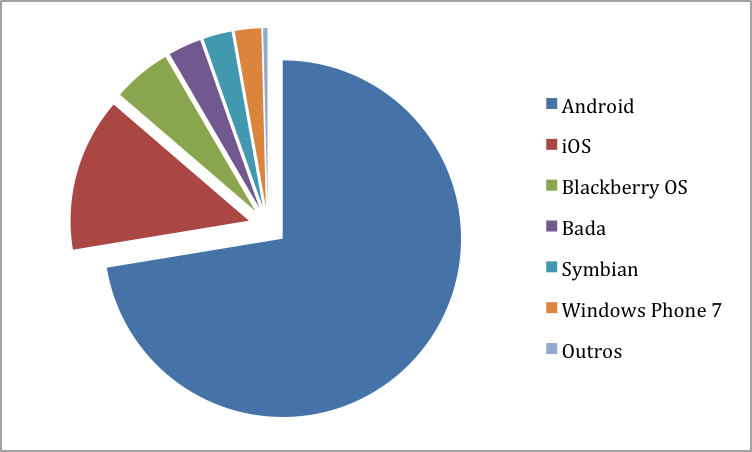
\includegraphics[width=0.8\linewidth]{figs/smartpizza.png}\\
   \caption{ MarketShare Q3 2012}
   \label{FIG:smartpizza}
 \end{figure}
 Fonte: \cite{neowin}
 
 Notadamente, o Android e o iOS são as plataformas mais populares. O grande diferencial entre o marketshare desses dois sistemas são o segmento de mercado: enquanto o Android atua em todos os segmentos, desde celulares \emph{low-end} aos celulares de ponta, o iOS atua somente com celulares de ponta, chamados \emph{high-end}. Outro fato a considerar é que, nesse gráfico, não são considerados outros dispositivos, como tocadores de música e \emph{tablets}.

 \section{iOS}
 \subsection{Visão Geral}

 O iOS é um sistema operacional para dispositivos móveis, lançado pela Apple em 2007. Inicialmente, foi desenvolvido para o iPhone, sendo posteriormente aproveitado nos dispositivos iPod Touch, iPad e Apple TV. Ele é um sistema operacional licenciado para rodar apenas em hardware produzido pela Apple, otimizado para a arquitetura de processadores ARM.
 
 Sua entrada de dados é feita de forma direta, através de multi- toques. Esses toques podem ser desde encostar o dedo, similar a um clique do mouse, até balançar o aparelho, de modo a utilizar seu acelerômetro. Todos os controles de entrada de dados são controlados pela \ac{GUI} Cocoa Touch.
 
 O livro \cite{usecabecaiphone} cita que o iPhone revolucionou a maneira de ver um celular: ele é, atualmente, uma plataforma de jogos, um organizador pessoal, um navegador (browser) completo e, claro, um celular. Muito de seu sucesso deve-se ao sucesso da loja virtual ``App Store'', de mídias e aplicativos, que abriu oportunidade para desenvolvedores independentes competirem em escala mundial com grandes empresas de software. 

 \subsection{Linguagem: Objective-c}
 A programação nativa em iOS utiliza uma linguagem de programação chamada Objective-C, com o \emph{framework} Foundation. 
 
 O Objective-C é uma linguagem de programação reflexiva e orientada a objeto, com origens no SmallTalk e no C. Foi criada no início da década de 80 por Brad Cox e Tom Love, mas somente se tornou popular quando foi licenciada pela NeXT, de Steve Jobs, em 1988. Atualmente é a principal linguagem utilizada para desenvolvimento para Mac OS X.
 
 Como o Objective-C foi construido sobre C, qualquer código C pode ser compilado com um compilador Objective-C. Por definição, é uma camada sobre o C que aceita orientação a objetos, através de mensagens.
 
 Em linguagens com ``message parsing'', métodos não são chamados de objetos, mas sim mensagens são enviadas ao objeto. Essa diferença implica em como o código referenciado pelo método ou nome da mensagem é executado. Em nosso caso, o ``alvo'' da mensagem é resolvido em tempo de execução, com o objeto receptor interpretando a mensagem.

 \subsection{Ciclo de vida}
 O ciclo de vida constitui uma sequência de eventos entre o início e a finalização da aplicação. Um aplicativo iOS começa quando o usuário toca o ícone da mesma na home do dispositivo. Feito isso, o sistema operacional inicia alguns procedimentos de renderização e chama a função principal (main.m) do aplicativo.
 
 Uma vez iniciado, o comando da execução passa a ser do UIKit, \emph{framework} de controle do iOS, que carrega a interface gráfica e lê o loop de eventos. Durante o loop, o UIKit delega cada evento a seu respectivo objeto e responde aos comandos emitidos pelo aplicativo. Quando o usuário realiza uma ação que causa um evento de saída, o UIKit notifica a aplicação e inicia o processo de saída.


 \section{Android}

 \subsection{Visão Geral}
 	O Android é a resposta do Google para ocupar o segmento de mercado de sistemas operacionais para plataformas móveis. Consiste em um novo sistema baseado no sistema operacional Linux, com diversas aplicações já instaladas, além de um ambiente de desenvolvimento forte e flexível. 
	
 	De acordo com \cite{lecheta}, o Android causou um grande impacto quando foi anunciado, em especial pelas empresas que estavam por trás de seu desenvolvimento: Google, Motorola, LG, Samsung, Sony, entre muitas outras. A esse grupo de empresas, denominado \ac{OHA}, coube à padronização de uma plataforma de código aberto e livre para celulares, com o objetivo de atender a demanda do mercado atual.
	
 	Um dos pontos fortes do Android é seu sistema flexível: é fácil integrar aplicações nativas com a sua aplicação, ou até mesmo substituir algumas dessas aplicações nativas pela sua própria. Isso gera um grande apelo para empresas de telefonia, que podem usar dessa personalização para lançarem suas próprias versões de aparelhos Android personalizados.
	
 	O grande foco do sistema é a interação entre aplicativos: agenda, maps, contatos são facilmente alcançáveis por qualquer aplicação. Essa funcionalidade é realizada por um recurso chamado Intent.%, que será abordado em capítulos posteriores.
	
 	Outro ponto forte do Android é que seu sistema operacional é baseado no Linux (baseado no kernel 2.6), ou seja, ele mesmo se encarrega de gerenciar a memoria em uso e os processos. Isso faz com que seja possível rodar mais de uma aplicação (genuinamente) ao mesmo tempo, fazendo com que outros aplicativos rodem em segundo plano durante outros serviços, como ao atender um telefonema ou acessar a internet.  
	
 	O que é dito como vantagem também é apontado, fatalmente, como um problema: uma vez que aplicativos podem rodar em segundo plano, aplicativos maliciosos também podem ser rodados em segundo plano. Durante muito tempo, aplicativos desse tipo podiam ser encontrados para download no Android Market (atualmente Google Play), havendo hoje uma melhor seleção dos aplicativos que de fato estão sendo disponibilizados na loja.

 \subsection{Linguagem: Java} 
 	A linguagem nativa de programação para Android é o Java, utilizando o \emph{framework} Android criado pela \ac{OHA}.
 	O Java é uma linguagem de propósito geral, concorrente e orientada a objetos. Sua primeira versão foi lançada em 1995 pela Sun Microsystems e, atualmente, encontra-se em sua sétima versão, sendo mantida pela Oracle. 
	
 	Atualmente, é uma das linguagens de programação mais populares do mundo, ocupando o 2º lugar no índice TIOBE. Devido a isso, há um grande número de desenvolvedores que possuem o pré-requisito básico para iniciar programação para Android: o domínio da linguagem.
	
 	O grande sucesso do Java é normalmente creditado a sua capacidade de funcionar nos mais diversos ambientes, desde micro-sistemas como cartões de crédito a grandes plataformas web. Isso é devido a implementação de sua máquina virtual, que é capaz de rodar nas mais diversas plataformas. 


 \subsection{Ciclo de vida}
 	 O ciclo de vida de uma aplicação Android é controlado por uma Activity, a qual também gerencia a interface com o usuário, recebe requisições, realiza o tratamento e processa.
	 
 	Toda Activity possui os seguintes métodos de controle, a saber:
 \begin{itemize}
 \item onCreate(): é o primeiro método a ser executado em uma Activity. Usualmente é o método responsável por carregar os layouts XML e inicializar atributos de classe e outros serviços.
 \item onStart(): é chamado imediatamente chamado após o onCreate(). Diferentemente deste, é chamado toda vez que a Activity volta a ter foco após um período em background.
 \item onResume(): Assim como o onStart(), é chamado no início da Activity e, também, quando a mesma volta a ter foco. A diferença entre ambos é que o onStart() só é invocado quando a Activity não está mais visível, enquanto o onResume() é chamado toda vez que retorna o foco.
 \item onPause(): é a primeira função a ser chamada quando a Activity perde o foco.
 \item onStop(): é chamado quando uma Activity é substituída por outra Activity
 \item onDestroy(): é o último método a ser executado. Quando o onDestroy() é executado, a Activity é considerada ``morta'' e fica pronta para ser removida pelo Garbage Collector.
 \item	onRestart(): Chamado quando a Activity sai do estado de ``stop''; após sua execução, é chamado o método onStart().
 \end{itemize}

 %\section{Redes Sociais}  será que vale mesmo a pena falar sobre isso?
 \section{Resumo do Capítulo}

 	Neste capítulo foram abordadas as três principais tecnologias necessárias para o desenvolvimento deste projeto: computação em nuvem, web services e computação móvel. Tais tecnologias foram aprofundadas em um nível o qual fornecessem ao leitor os pré-requisitos para a compreensão do restante do projeto, o qual será apresentado nos capítulos posteriores.
 
